%=========================================================
%               CLASSE DU DOCUMENT
%=========================================================
\documentclass[12pt,a4paper]{article}

%=========================================================
%         ENCODAGE ET POLICES DE CARACTÈRES
%=========================================================
\usepackage[utf8]{inputenc}    % Encodage UTF-8 (inutile avec XeLaTeX/LuaLaTeX)
\usepackage[T1]{fontenc}       % Meilleure gestion des caractères accentués
\usepackage{lmodern}           % Police Latin Modern
\usepackage{times}             % Police Times (à supprimer si tu préfères Latin Modern)

%=========================================================
%                MATHÉMATIQUES
%=========================================================
\usepackage{amsmath}           % Environnements mathématiques avancés
\usepackage{amssymb}           % Symboles mathématiques supplémentaires
\usepackage{amsfonts}          % Polices mathématiques
\usepackage{mathrsfs}          % Police calligraphique (\mathscr)
\usepackage{tkz-tab}           % Tableaux de signes et de variations
\everymath{\displaystyle}      % Affiche toutes les formules en style "display"

%=========================================================
%               MISE EN PAGE
%=========================================================
\usepackage[
    left=1cm,
    right=1cm,
    top=1cm,
    bottom=1.7cm
]{geometry}                    % Marges du document

\usepackage{multicol}          % Texte sur plusieurs colonnes
\usepackage{float}             % Placement précis des figures et tableaux

%=========================================================
%            TABLEAUX ET LISTES
%=========================================================
\usepackage{array}             % Colonnes de tableaux personnalisées
\usepackage{multirow}          % Fusion de lignes dans les tableaux
\usepackage{enumitem}          % Personnalisation des listes

\usepackage{tikz}
\usetikzlibrary{angles,quotes,arrows.meta}
%=========================================================
%            COULEURS ET BOÎTES
%=========================================================
\usepackage[most]{tcolorbox}   % Boîtes colorées très personnalisables
\tcbuselibrary{skins,hooks}    % Bibliothèques supplémentaires de tcolorbox

\usepackage{mdframed}          % Cadres autour de paragraphes
\usepackage{varwidth}          % Largeur automatique des boîtes

%=========================================================
%                DESSINS ET GRAPHIQUES
%=========================================================
\usepackage{tikz}              % Dessins vectoriels
\usetikzlibrary{calc}
\usetikzlibrary{
    arrows,
    shapes.geometric,
    fit,
    patterns
}

\usepackage{pgfplots}          % Tracés de fonctions et graphiques
\pgfplotsset{compat=1.15}

%=========================================================
%              LIENS HYPERTEXTES
%=========================================================
\usepackage[
    colorlinks=true,
    linkcolor=blue,
    urlcolor=blue,
    citecolor=blue
]{hyperref}

%=========================================================
%          ÉLÉMENTS EN ARRIÈRE-PLAN
%=========================================================
\usepackage{eso-pic}           % Ajout de filigranes ou d'éléments sur chaque page

%=========================================================
%              SYMBOLES DIVERS
%=========================================================
\usepackage{pifont}            % Symboles (✓, ✗, etc.)

\DeclareUnicodeCharacter{2460}{\text{\ding{172}}} % Pour ①
\DeclareUnicodeCharacter{2461}{\text{\ding{173}}} % Pour ②
%=========================================================
%      PERSONNALISATION DES LISTES NUMÉROTÉES
%=========================================================

\newcommand\circitem[1]{%
\tikz[baseline=(char.base)]{
\node[circle,draw=gray,fill=red!55,
minimum size=1.2em,inner sep=0] (char) {#1};}}

\newcommand\boxitem[1]{%
\tikz[baseline=(char.base)]{
\node[fill=cyan,
minimum size=1.2em,inner sep=0] (char) {#1};}}

\setlist[enumerate,1]{label=\protect\circitem{\arabic*}}
\setlist[enumerate,2]{label=\protect\boxitem{\alph*}}

%=========================================================
%            COMMANDES PERSONNALISÉES
%=========================================================

% Soulignement coloré
\newcommand{\myul}[2][black]{%
\setulcolor{#1}\ul{#2}\setulcolor{black}}

% Tabulation horizontale
\newcommand\tab[1][1cm]{\hspace*{#1}}

%=========================================================
%             COMPTEURS PERSONNALISÉS
%=========================================================

%---------- Exemple ----------
\newcounter{exemple}

\newcommand{\exemple}{%
\refstepcounter{exemple}
\textbf{\textcolor{orange}{Exemple \theexemple : }}
\ignorespaces}

%---------- Solution ----------
\newcounter{solution}

\newcommand{\solution}{%
\refstepcounter{solution}
\textbf{\textcolor{orange}{Solution \thesolution : }}
\ignorespaces}

%---------- Exercices ----------
\definecolor{myorange}{rgb}{1.0,0.8,0.0}

\newcounter{exerciceapp}

\newcommand{\exerciceapp}{%
\refstepcounter{exerciceapp}
\textbf{\textcolor{myorange}
{Exercice d'application \theexerciceapp : }}
\ignorespaces}

%---------- Corrections ----------
\newcounter{correction}

\newcommand{\correction}{%
\refstepcounter{correction}
\textbf{\textcolor{myorange}
{Correction \thecorrection : }}
\ignorespaces}

%---------- Remarques ----------
\definecolor{myorange1}{rgb}{1.0,1.0,0.0}
\usepackage{enumitem}

\definecolor{myred}{RGB}{180, 40, 40}
\definecolor{myblue}{RGB}{20, 50, 120}
\newcounter{remarque}

\newcommand{\remarque}{%
\refstepcounter{remarque}
\textbf{\textcolor{myorange1}
{Remarque \theremarque : }}
\ignorespaces}

%=========================================================
%                 FILIGRANE
%=========================================================

\AddToShipoutPicture{
    \AtTextCenter{
        \makebox[0pt]{
            \rotatebox{45}{
                \textcolor[gray]{0.6}{
                    \fontsize{5cm}{5cm}\selectfont PGB
                }
            }
        }
    }
}

\begin{document}
% En-tête personnalisée
\begin{center}
    \Large\textbf{\underline{\textcolor{red}{Équations et Inéquations Du second dégré}}}\\[-0.1cm]
    \normalsize\textbf{Prof : M. BA} \hfill \textbf{Classe : 1erS2}\\[-0.1cm]
    \textbf{Année scolaire : 2025 -- 2026}
\end{center}
%=========================================================

\vspace{1em}

% ========================================================================
% PARTIE I : ÉQUATIONS DU SECOND DEGRÉ
% ========================================================================
\section*{\color{myred} I) Equations du second degré}

\subsection*{\color{myred} 1) Définition}
Une équation du second degré à une inconnue $x$ est une équation qui peut se mettre sous la forme :
\[
ax^2 + bx + c = 0
\]
où $a$, $b$ et $c$ sont des nombres réels, avec $a \neq 0$.

On appelle \textbf{trinôme du second degré} l'expression $ax^2 + bx + c$.

\subsection*{\color{myred} 2) Méthodes de résolutions}

\subsubsection*{\color{myred} a) Équation du type $ax^2 + bx = 0$ où $a \neq 0$ et $b \neq 0$}
On factorise par $x$ :
\[
ax^2 + bx = 0 \iff x(ax + b) = 0
\]
Un produit de facteurs est nul si et seulement si l'un des facteurs est nul, donc :
\[
x = 0 \quad \text{ou} \quad ax + b = 0 \iff x = -\frac{b}{a}
\]
\textbf{Conclusion :} Les solutions sont $S = \left\{0, -\dfrac{b}{a}\right\}$.

\begin{itemize}
    \item \textbf{Exemple :} Résoudre $2x^2 - 6x = 0$.
    \[
    2x^2 - 6x = 0 \iff 2x(x-3) = 0
    \]
    Donc $x=0$ ou $x=3$. \quad $S = \{0, 3\}$.
\end{itemize}

\subsubsection*{\color{myred} b) Équation du type $ax^2 + c = 0$ où $a \neq 0$ et $c \neq 0$}
On isole $x^2$ :
\[
ax^2 + c = 0 \iff x^2 = -\frac{c}{a}
\]
Trois cas se présentent :
\begin{itemize}
    \item Si $-\dfrac{c}{a} > 0$, alors $x = \pm \sqrt{-\dfrac{c}{a}}$.
    \item Si $-\dfrac{c}{a} = 0$, alors $x = 0$ (mais ce cas n'est pas possible ici car $c \neq 0$).
    \item Si $-\dfrac{c}{a} < 0$, alors il n'y a pas de solution réelle.
\end{itemize}

\begin{itemize}
    \item \textbf{Exemples :}
    \begin{enumerate}[label=\arabic*)]
        \item $3x^2 - 12 = 0 \iff x^2 = 4 \iff x = \pm 2$. \quad $S = \{-2, 2\}$.
        \item $2x^2 + 8 = 0 \iff x^2 = -4$ : pas de solution réelle. \quad $S = \emptyset$.
    \end{enumerate}
\end{itemize}

\subsubsection*{\color{myred} c) Cas général : équation du type $ax^2 + bx + c = 0$ où $a \neq 0$}

\paragraph*{\color{myred} Forme canonique du trinôme du second degré}
Pour tout trinôme du second degré $ax^2 + bx + c$ (avec $a \neq 0$), il existe une forme dite \textbf{canonique} :
\[
ax^2 + bx + c = a\left(x + \dfrac{b}{2a}\right)^2 - \dfrac{b^2 - 4ac}{4a}
\]
Ou encore :
\[
ax^2 + bx + c = a\left(x + \dfrac{b}{2a}\right)^2 - \dfrac{\Delta}{4a}
\]
où l'on pose $\Delta = b^2 - 4ac$ (appelé \textbf{discriminant}).

\begin{itemize}
    \item \textbf{Exemple :} Mettre $2x^2 - 8x + 6$ sous forme canonique.
    \[
    2x^2 - 8x + 6 = 2(x^2 - 4x) + 6 = 2\left[(x-2)^2 - 4\right] + 6
    = 2(x-2)^2 - 8 + 6 = 2(x-2)^2 - 2.
    \]
    On a bien $\Delta = (-8)^2 - 4 \times 2 \times 6 = 64 - 48 = 16$, et $-\dfrac{\Delta}{4a} = -\dfrac{16}{8} = -2$.
\end{itemize}

\paragraph*{\color{myred} Forme factorisée d'un trinôme du second degré}
La forme factorisée d'un trinôme dépend du signe de $\Delta = b^2 - 4ac$ :

\begin{itemize}
    \item Si $\Delta > 0$ : le trinôme admet deux racines réelles distinctes
    \[
    x_1 = \dfrac{-b - \sqrt{\Delta}}{2a} \quad \text{et} \quad x_2 = \dfrac{-b + \sqrt{\Delta}}{2a}
    \]
    et la factorisation est :
    \[
    ax^2 + bx + c = a(x - x_1)(x - x_2)
    \]
    
    \item Si $\Delta = 0$ : le trinôme admet une racine double
    \[
    x_0 = -\dfrac{b}{2a}
    \]
    et la factorisation est :
    \[
    ax^2 + bx + c = a(x - x_0)^2
    \]
    
    \item Si $\Delta < 0$ : le trinôme n'admet pas de racine réelle et ne se factorise pas dans $\mathbb{R}$.
\end{itemize}

\subsection*{\color{myred} 3) Résolution de l'équation $ax^2 + bx + c = 0$ où $a \neq 0$}
Pour résoudre une équation du second degré, on procède comme suit :

\begin{enumerate}
    \item On calcule le discriminant $\Delta = b^2 - 4ac$.
    \item On distingue trois cas :
    \begin{itemize}
        \item Si $\Delta > 0$ : deux solutions réelles :
        \[
        x_1 = \dfrac{-b - \sqrt{\Delta}}{2a} \quad \text{et} \quad x_2 = \dfrac{-b + \sqrt{\Delta}}{2a}
        \]
        \item Si $\Delta = 0$ : une solution double :
        \[
        x_0 = -\dfrac{b}{2a}
        \]
        \item Si $\Delta < 0$ : aucune solution réelle ($S = \emptyset$).
    \end{itemize}
\end{enumerate}

\begin{itemize}
    \item \textbf{Exemples :}
    \begin{enumerate}[label=\arabic*)]
        \item Résoudre $x^2 - 5x + 6 = 0$.
        
        $\Delta = (-5)^2 - 4 \times 1 \times 6 = 25 - 24 = 1 > 0$.
        \[
        x_1 = \dfrac{5 - \sqrt{1}}{2} = \dfrac{5-1}{2} = 2, \quad
        x_2 = \dfrac{5 + \sqrt{1}}{2} = \dfrac{5+1}{2} = 3
        \]
        $S = \{2, 3\}$.
        
        \item Résoudre $x^2 + 4x + 4 = 0$.
        
        $\Delta = 4^2 - 4 \times 1 \times 4 = 16 - 16 = 0$.
        \[
        x_0 = -\dfrac{4}{2} = -2
        \]
        $S = \{-2\}$.
        
        \item Résoudre $x^2 + x + 1 = 0$.
        
        $\Delta = 1^2 - 4 \times 1 \times 1 = 1 - 4 = -3 < 0$.
        $S = \emptyset$.
    \end{enumerate}
\end{itemize}

\subsection*{\color{myred} 4) Somme et Produit des racines}

\subsubsection*{\color{myred} a) Propriété 1}
Si le trinôme $ax^2 + bx + c$ admet deux racines $x_1$ et $x_2$ (éventuellement confondues si $\Delta = 0$), alors :
\[
S = x_1 + x_2 = -\dfrac{b}{a} \quad \text{(somme des racines)}
\]
et
\[
P = x_1 \times x_2 = \dfrac{c}{a} \quad \text{(produit des racines)}
\]

\begin{itemize}
    \item \textbf{Exemple :} Pour l'équation $2x^2 - 6x + 4 = 0$, on a $\Delta = 4 > 0$, les racines sont $x_1 = 1$ et $x_2 = 2$.
    \[
    S = 1+2 = 3 = -\dfrac{-6}{2}, \quad P = 1 \times 2 = 2 = \dfrac{4}{2}.
    \]
\end{itemize}

\subsubsection*{\color{myred} b) Propriété 2}
Si deux réels $x$ et $y$ ont pour somme $S = x + y$ et pour produit $P = xy$, alors $x$ et $y$ sont les solutions de l'équation du second degré :
\[
X^2 - SX + P = 0
\]
où $X$ est l'inconnue.

\begin{itemize}
    \item \textbf{Exemple :} Trouver deux nombres dont la somme est 5 et le produit est 6.
    
    Ils sont solutions de $X^2 - 5X + 6 = 0$.
    On a $\Delta = 25 - 24 = 1 > 0$, donc :
    \[
    X_1 = \dfrac{5 - 1}{2} = 2, \quad X_2 = \dfrac{5 + 1}{2} = 3.
    \]
    Les deux nombres sont 2 et 3.
\end{itemize}

% ========================================================================
% PARTIE II : INÉQUATIONS DU SECOND DEGRÉ
% ========================================================================
\section*{\color{myred} II) Inéquation Du Second Dégré}

\subsection*{\color{myred} 1) Définition}
Une inéquation du second degré à une inconnue $x$ est une inéquation qui peut se mettre sous l'une des formes suivantes :
\[
ax^2 + bx + c \geq 0, \quad ax^2 + bx + c > 0, \quad ax^2 + bx + c \leq 0, \quad ax^2 + bx + c < 0
\]
où $a \neq 0$.

Résoudre une inéquation du second degré, c'est déterminer l'ensemble des réels $x$ pour lesquels l'inégalité est vraie.

\subsection*{\color{myred} 2) Signe d'un trinôme du second degré}
Le signe du trinôme $ax^2 + bx + c$ (avec $a \neq 0$) dépend du signe de $\Delta = b^2 - 4ac$ et du signe de $a$.

\paragraph*{\color{myred} Règle de signe :}

\begin{enumerate}
    \item \textbf{Si $\Delta < 0$ :} 
    Le trinôme est toujours du signe de $a$ (pour tout $x \in \mathbb{R}$).
     
\begin{center}
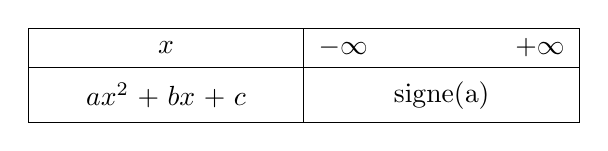
\begin{tikzpicture}[node style/.style={fill opacity=0,text opacity=1}]
    \tkzTabInit[
        lgt=3.5,
        espcl=2.5
    ]{$x$/.5,$ax^2 + bx + c$/.7}
    {$-\infty$ , $+\infty$}
    \tkzTabLine{,\text{signe(a)},}
\end{tikzpicture}
\end{center}

    \item \textbf{Si $\Delta = 0$ :}
    Le trinôme est du signe de $a$ pour tout $x \neq -\dfrac{b}{2a}$ et s'annule en $x_0 = -\dfrac{b}{2a}$.
    
    \begin{center}
    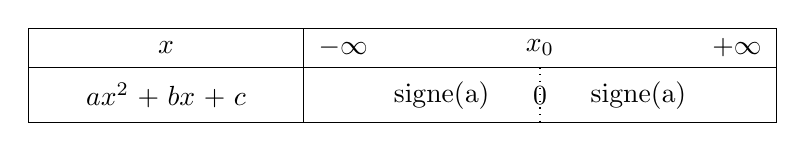
\begin{tikzpicture}[node style/.style={fill opacity=0,text opacity=1}]
    \tkzTabInit[
        lgt=3.5,
        espcl=2.5
    ]{$x$/.5,$ax^2 + bx + c$/.7}
    {$-\infty$,$x_0$,$+\infty$}
    \tkzTabLine{,\text{signe(a)},z,\text{signe(a)},}
    \end{tikzpicture}
    \end{center}

    \item \textbf{Si $\Delta > 0$ :}
    Le trinôme est du signe de $a$ à l'extérieur des racines (c'est-à-dire pour $x < x_1$ et $x > x_2$) et du signe de $-a$ entre les racines (pour $x_1 < x < x_2$).
    \begin{center}
    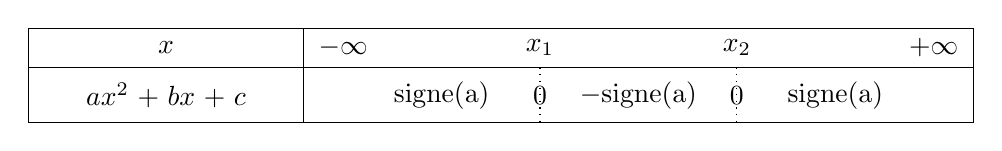
\begin{tikzpicture}[node style/.style={fill opacity=0,text opacity=1}]
    \tkzTabInit[
        lgt=3.5,
        espcl=2.5
    ]{$x$/.5,$ax^2 + bx + c$/.7}
    {$-\infty$,$x_1$,$x_2$,$+\infty$}
    \tkzTabLine{,\text{signe(a)},z,-\text{signe(a)},z,\text{signe(a)},}
    \end{tikzpicture}
    \end{center}
\end{enumerate}

\subsection*{\color{myred} 3) Résolution d'une inéquation du second degré à une inconnue $x$}
Pour résoudre une inéquation du second degré, on procède comme suit :
\begin{enumerate}
    \item On se ramène à la forme $ax^2 + bx + c \geq 0$ (ou $>0$, $\leq 0$, $<0$).
    \item On calcule le discriminant $\Delta$.
    \item On détermine les racines (si elles existent).
    \item On construit le tableau de signe du trinôme.
    \item On lit l'ensemble des solutions selon l'inégalité.
\end{enumerate}

\begin{itemize}
    \item \textbf{Exemples :}
    \begin{enumerate}[label=\arabic*)]
        \item Résoudre $x^2 - 5x + 6 \geq 0$.
        
        On a $\Delta = 1 > 0$, $a = 1 > 0$. Les racines sont $x_1 = 2$ et $x_2 = 3$.
        
        \textbf{Tableau de signe :}

    \begin{center}
    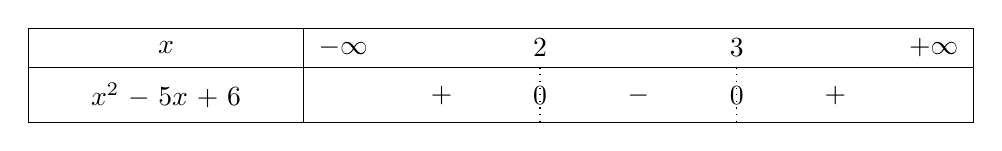
\begin{tikzpicture}[node style/.style={fill opacity=0,text opacity=1}]
    \tkzTabInit[
        lgt=3.5,
        espcl=2.5
    ]{$x$/.5,$x^2 - 5x + 6$/.7}
    {$-\infty$,$2$,$3$,$+\infty$}
    \tkzTabLine{,+,z,-,z,+,}
    \end{tikzpicture}
    \end{center}
        
        Donc $S = ]-\infty, 2] \cup [3, +\infty[$.
        
        \item Résoudre $-2x^2 + 8x - 6 > 0$.
        
        On multiplie par $-1$ (en changeant le sens de l'inégalité) : $2x^2 - 8x + 6 < 0$.
        On a $\Delta = 16 > 0$, $a = 2 > 0$. Les racines sont $x_1 = 1$ et $x_2 = 3$.
        
        \textbf{Tableau de signe de $2x^2 - 8x + 6$ :}

    \begin{center}
    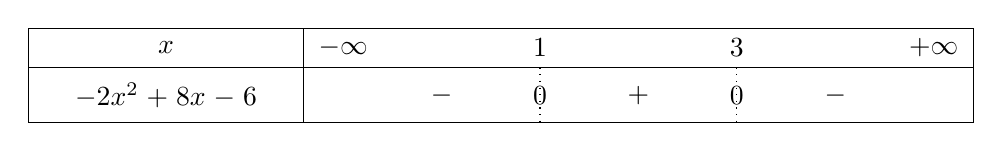
\begin{tikzpicture}[node style/.style={fill opacity=0,text opacity=1}]
    \tkzTabInit[
        lgt=3.5,
        espcl=2.5
    ]{$x$/.5,$-2x^2 + 8x - 6$/.7}
    {$-\infty$,$1$,$3$,$+\infty$}
    \tkzTabLine{,-,z,+,z,-,}
    \end{tikzpicture}
    \end{center}
        
        On veut $2x^2 - 8x + 6 < 0$, donc $S = ]1, 3[$.
        
        \item Résoudre $x^2 + x + 1 < 0$.
        
        $\Delta = -3 < 0$ et $a = 1 > 0$, donc le trinôme est toujours $> 0$.
        L'inéquation $< 0$ n'a pas de solution : $S = \emptyset$.
        
        \item Résoudre $x^2 - 4x + 4 \leq 0$.
        
        $\Delta = 0$, $a = 1 > 0$. La racine double est $x_0 = 2$.
        
        \textbf{Tableau de signe :}
    \begin{center}
    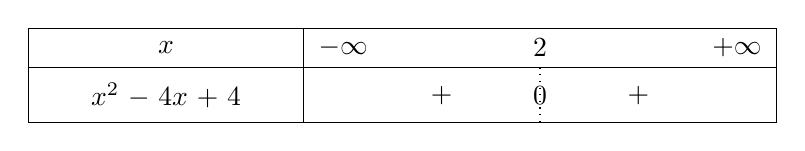
\begin{tikzpicture}[node style/.style={fill opacity=0,text opacity=1}]
    \tkzTabInit[
        lgt=3.5,
        espcl=2.5
    ]{$x$/.5,$x^2 - 4x + 4$/.7}
    {$-\infty$,$2$,$+\infty$}
    \tkzTabLine{,+,z,+,}
    \end{tikzpicture}
    \end{center}
        
        Le trinôme est $> 0$ pour $x \neq 2$ et s'annule en $2$.
        Donc $S = \{2\}$.
    \end{enumerate}
\end{itemize}

% ========================================================================
% RÉSUMÉ
% ========================================================================
\newpage
\section*{\color{myred} RÉSUMÉ DES CAS POSSIBLES}

\subsection*{\color{myred} Tableau récapitulatif :}

\begin{center}
\renewcommand{\arraystretch}{1.5}
\begin{tabular}{|c|c|c|c|c|}
\hline
$\Delta$ & $a$ & $ax^2+bx+c=0$ & $ax^2+bx+c>0$ & $ax^2+bx+c<0$ \\
\hline
$\Delta > 0$ & $a>0$ & $\{x_1, x_2\}$ & $]-\infty, x_1[ \cup ]x_2, +\infty[$ & $]x_1, x_2[$ \\
\hline
$\Delta > 0$ & $a<0$ & $\{x_1, x_2\}$ & $]x_1, x_2[$ & $]-\infty, x_1[ \cup ]x_2, +\infty[$ \\
\hline
$\Delta = 0$ & $a>0$ & $\{x_0\}$ & $\mathbb{R} \setminus \{x_0\}$ & $\emptyset$ \\
\hline
$\Delta = 0$ & $a<0$ & $\{x_0\}$ & $\emptyset$ & $\mathbb{R} \setminus \{x_0\}$ \\
\hline
$\Delta < 0$ & $a>0$ & $\emptyset$ & $\mathbb{R}$ & $\emptyset$ \\
\hline
$\Delta < 0$ & $a<0$ & $\emptyset$ & $\emptyset$ & $\mathbb{R}$ \\
\hline
\end{tabular}
\end{center}

\vspace{1em}
\noindent \textbf{Remarque :} Pour les inéquations avec $\geq$ ou $\leq$, on inclut les racines (si elles existent) dans les intervalles de solutions.

% ========================================================================
% EXERCICES D'APPLICATION
% ========================================================================
\newpage
\section*{\color{myred} EXERCICES D'APPLICATION}

\subsection*{\color{myred} Exercice 1 : Équations}
Résoudre dans $\mathbb{R}$ les équations suivantes :
\begin{enumerate}[label=\alph*)]
    \item $x^2 - 7x + 12 = 0$
    \item $2x^2 + 5x - 3 = 0$
    \item $x^2 - 6x + 9 = 0$
    \item $x^2 + 2x + 5 = 0$
    \item $3x^2 - 5x = 0$
    \item $4x^2 - 9 = 0$
\end{enumerate}

\subsection*{\color{myred} Exercice 2 : Inéquations}
Résoudre dans $\mathbb{R}$ les inéquations suivantes :
\begin{enumerate}[label=\alph*)]
    \item $x^2 - 4x + 3 > 0$
    \item $-x^2 + 3x + 4 \geq 0$
    \item $2x^2 - 8x + 8 < 0$
    \item $x^2 + x + 1 \leq 0$
    \item $x^2 - 4x + 4 \geq 0$
    \item $-3x^2 + 6x - 3 \leq 0$
\end{enumerate}

\subsection*{\color{myred} Exercice 3 : Synthèse}
Soit $f(x) = x^2 - 4x + 3$.
\begin{enumerate}[label=\arabic*)]
    \item Déterminer le domaine de définition de $f$.
    \item Résoudre $f(x) = 0$.
    \item Factoriser $f(x)$.
    \item Étudier le signe de $f(x)$ et donner le tableau de signe avec TikZ.
    \item Résoudre $f(x) > 0$ et $f(x) \leq 0$.
\end{enumerate}

\subsection*{\color{myred} Exercice 4 : Problème}
Un rectangle a pour longueur $x+3$ et pour largeur $x-1$ (où $x > 1$).
\begin{enumerate}[label=\arabic*)]
    \item Exprimer l'aire du rectangle en fonction de $x$.
    \item Pour quelles valeurs de $x$ l'aire est-elle égale à $15$ ?
    \item Pour quelles valeurs de $x$ l'aire est-elle strictement supérieure à $8$ ?
\end{enumerate}
\end{document}